\documentclass[12pt,journal,compsoc,onecolumn]{IEEEtran}
\newcommand\MYhyperrefoptions{bookmarks=true,bookmarksnumbered=true,
pdfpagemode={UseOutlines},plainpages=false,pdfpagelabels=true,
colorlinks=true,linkcolor={black},citecolor={black},pagecolor={black},
urlcolor={black},
pdftitle={Midterm Review},%<!CHANGE!
pdfsubject={Typesetting},%<!CHANGE!
pdfauthor={Cecil Li},%<!CHANGE!
pdfkeywords={Computer Society, IEEEtran, journal, LaTeX, paper,
             template}}%<^!CHANGE!
\usepackage{pdfpages}
\usepackage{float}
\usepackage[center]{caption}
\usepackage{amsmath}
\usepackage{listings}
\usepackage{longtable}
\usepackage{changepage}
\usepackage{subcaption}

\lstset{breaklines=true} 
\lstset{numbers=left, numberstyle=\scriptsize\ttfamily, numbersep=10pt, captionpos=b} 
\definecolor{gray-5}{gray}{0.9}
\lstset{backgroundcolor=\color{gray-5}}
\lstset{basicstyle=\small\ttfamily}
\lstset{framesep=4pt}
\newcommand{\inlineCode}{\lstinline[basicstyle=\normalsize\ttfamily]}

\pagestyle{headings}
\begin{document}
\title{Continental Scale Heterogeneous Knowledge Integration for Expert Agricultural Decision Support System\\ \vspace{1cm} Project Midterm Review}
\author{Student: Cecil Li, u4646865\\Primary supervisor: Dr. Ritaban Dutta, CSIRO\\ University supervisor: Dr. Jon Kim, ANU}

% The paper headers
\markboth{Cecil Li u4646865\hspace{6cm}Midterm Review}{}
% make the title area
\maketitle

\newpage
\vspace*{\fill}
\begin{center}
\section*{Acknowledgment}
\end{center}
\begin{adjustwidth}{2cm}{2cm}
I wish to thank my supervisor Dr. Ritaban Dutta for continuously supervising my work and providing insightful guidance. The CSIRO Computational Informatics, Hobart and the Tasmanian node of the Australian Centre for Broadband Innovation is providing the full support for my individual project. The
cosmic ray sensor data was made available through the CosmOz
Australian soil moisture monitoring network funded by CSIRO
and deployed by Aaron Hawdon and Rex Keen of CSIRO Land
and Water, Townsville, Australia. Soil samples for sensor
calibration were collected by Bill Cotching of Tasmanian
Institute of Agriculture. Data were delivered through CSIRO
data service system developed by Peter Taylor. I would
like to thank Peter Briggs and Simon Lovell for providing access
to the AWAP database and SILO database. I would also like to acknowledge the use of FIRMS data and imagery from the Land Atmosphere Near-real time Capability for EOS (LANCE) system operated by the NASA/GSFC/Earth Science Data and Information System (ESDIS) with funding provided by NASA/HQ
\end{adjustwidth}
\vspace*{\fill}
\newpage

\vspace*{\fill}
\begin{abstract}\normalsize 
Australia, despite being the 6th largest country of total area in the world, its water scarcity still a heated issue unresolved. Primarily in the agricultural sector, which accounts for 60\% of the total water consumption nationwide. This study aims to develop an intelligent decision support system assisting in irrigation planning for the farming industry. The system integrates multiple data from different sources including but not limit to Bureau of Meteorology of Australia and National Aeronautics and Space Administration of the United States. In this study, various machine learning techniques are applied and tested to achieve optimal results, which then being delivered to the users in a visual manner via state-of-the-art mobile applications based on the Android OS, of which the work has been published and presented in an IEEE Conference in Baltimore, MD, USA in November 2013(Li et al 2013\cite{Li2013}).  A more sophisticated and novel analysis is also discussed in this study, to explore the viability of using data-driven approach to model the impact of environmental change of any arbitrary region.
\end{abstract}
\tableofcontents

\vspace*{\fill}
\newpage
\section{Introduction}
Australia, despite being the 6th largest country in the world, area-wise speaking. Its water resources are heavily limited in the regions where the population and agricultural activities are concentrated. In the most recent Water Account Report released by Australian Bureau of Statistics (2013\cite{Statistics2013}), it is found that a total amount of around 75,000 GL of water was extracted and used within the Australian economy. Among which, the actual total consumption was 16,000 GL, a 20\% increase from the previous annum. The agricultural sector alone accounted for 9,418 GL, or 59\% of total water consumption, mainly for irrigation usage.\\
\newline
From the farming industry's point of view, proper planning of irrigation is also a significant issue to solve, due to the scarcity of water supply and highly priced electricity for operating irrigation systems, as well as the fact that excessive water in the soil could cause fungal infection in the plants\cite{Wong1984}, which results in reduced yields. Thus, a low-cost solution is needed to provide reliable advices on irrigation planning for the farmers in Australia so that wastage and costs can both be minimized. \\
\newline
One solution to the problem is to combine field experiments with conventional water balance modeling. However, field experiments are relatively expensive to conduct and has its limitations on specific land conditions, which means that it would be impractical to generalise the water balance estimation entirely on field experiment results. There is a need for on demand complementary knowledge integration from multiple data sources to increase efficiency and automatic interpretation of the knowledge.\\
\newline
This thesis explores the possibility of producing most probable high resolution prediction regarding the water balance in any region within Australia by implementing an intelligent system that can integrate multiple spatio-temporal data from various independent sensors and models, based on scientific foundation rather than human intuition.\\
\newline
In this thesis, a point-based approach is first implemented. Of which, a novel knowledge integration and machine learning analysis based water usage recommendation system has been investigated and proposed based on the CSIRO Sensor Cloud. To demonstrate the outcome, an Android OS based recommendation framework is developed for the purpose.\\
\newline
After validating the viability of such system, an area-wise approach is further developed. In this study, the novelty lies in where multiple points in a certain area are used to develop the Machine Learning model so that the limitation of conventional water balance model can be overcome by a data driven approach. 

\section{The Water Balance Model}
A system can be one of several hydrological domains, such as a column of soil, or a drainage basin. Water balance can also refer to the ways in which an organism maintains water in dry or hot conditions. It is often discussed in reference to plants or arthropods, which have a variety of water retention mechanisms, including a lipid waxy coating that has limited permeability.\\
\newline
Water balance is based on the law of conservation of mass:
any change in the water content of a given soil volume during a specified period must equal the difference between the amount of water added to the soil volume and the amount of water withdrawn from it.
	\begin{figure}[H]
		\begin{center} 
		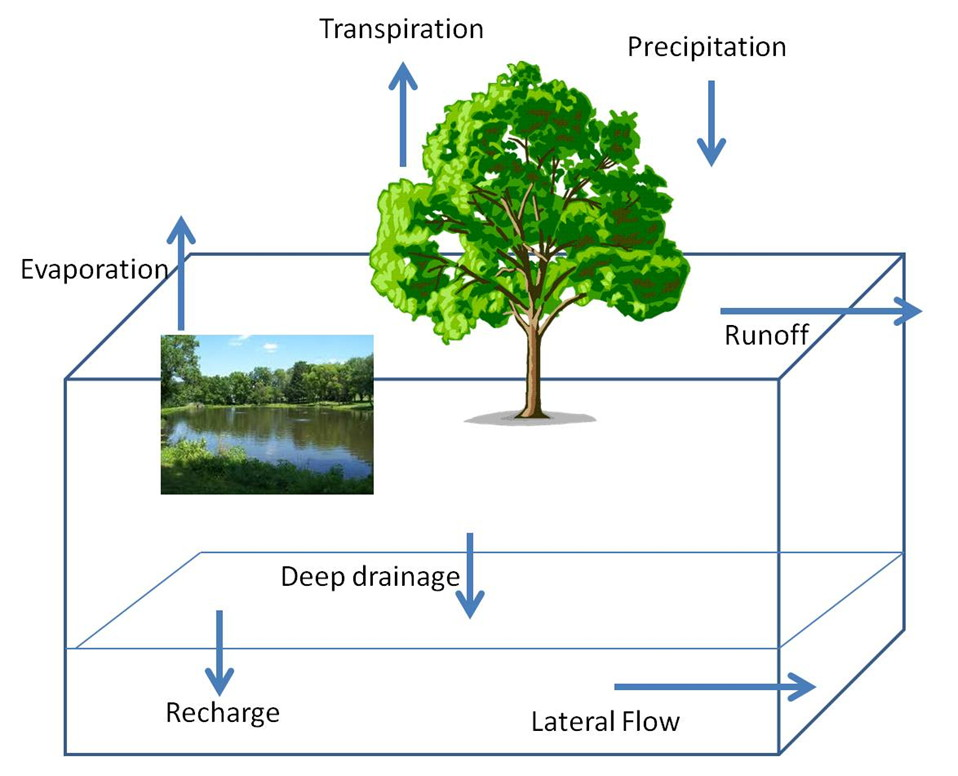
\includegraphics[width=12cm]{waterbalance.jpg}
		\caption{Illustration of the Water Balance Model}
		\label{fig:wbillustration}
		\end{center}
	\end{figure}
The root zone water balance is usually expressed as:
	\begin{align}
	\Delta S &= P - E-T-RO-DD
	\label{eq:wbequation}
	\end{align}
Where $\Delta S$ is the change in root zone soil water storage over the time period of interest, $P$ is precipitation that get to the soil, $E$ is direct evaporation from the soil and water body surface, $T$ is transpiration by plants and grass, $RO$ is surface runoff or overland flow, and $DD$ is deep drainage out of the root zone.\\
\newline
When the control volume is the entire catchment represented by given latitude and longitude information, the surface water balance equation can be expressed as:
\begin{align}
	\Delta <S> &= <P> - <ET>-<Q>-<R>
	\label{eq:wbsimple}
\end{align}
Where $\Delta <S>$ is the change in spatially averaged catchment water storage,
$<P>$ is spatially averaged precipitation, $<ET>$ is the spatially averaged catchment
evapotranspiration, $<Q>$ is the spatially averaged catchment surface runoff, and $<R>$
is the spatially averaged catchment recharge. Equation \ref{eq:wbsimple} was used for the historic water balance calculation. A multi data source based ''Water Balance Ontology'' is created to represent this model in a machine readable structure.
\begin{quote}
	\begin{lstlisting}
Simplified Model for Catchment
Catchment Surface Water Balance Equation (Control Volume is the entire catchment)

d<S> = <P> - <ET> - <Q> - <R>
      = SOIL MOISTURE = {MsoilUL AWAP // MsoilULagg AWAP // MsoilLL AWAP // MsoilLLagg AWAP}

d<S> = change in spatially averaged catchment water storage = ZERO Ideally when balance is perfect
<P> = spatially averaged precipitation {rain AWAP}
<ET> = spatially averaged evapotranspiration {Evap(soil+veg) AWAP  +  OpenWaEvap AWAP}
<Q> = spatially averaged catchment surface runoff {SurfRun AWAP}
<R> = spatially averaged catchment rechage {DeepDrain AWAP} while Sub-surface flow is considered zero.
	\end{lstlisting}\label{quote:wb}
\end{quote}
Additionally, an irrigation water usage indicator is calculated for a clear representation of soil moisture level.
\begin{quote}
	\begin{lstlisting}
Conditional Rule:
d<Irrigation Water Requirement Indicator>
	=<P> - <ET> - <Q> - <R>- d<S>
	= positive if above catchment water storage capacity = Class 1
	= negative if below catchment water storage capacity = Class 2
	= Zero if ideal balanced situation
	\end{lstlisting}\label{quote:wb2}
\end{quote}
\section{The Datasets}
The implemented system integrates multiple data sources of various types, as listed in Table \ref{table:datasources}
\begin{center}
\bgroup
\def\arraystretch{1.5}%
   \small \begin{longtable}{ | p{2cm} |p{2cm}  | p{2cm}  | p{2cm}  | p{2cm}  | p{5cm} |}
    \hline
    Name& Abbreviation  & Provider & Spatial Resolution & Temporal Resolution & Notes \\ \hline
	Australian Water Availability Project & AWAP & The Bureau of Meteorology & 5km & Weekly & A derived product providing 18 variables including Soil Moisture, Rainfall, Runoff etc.\cite{Raupach2009} \\ \hline
	Australian National Cosmic Ray Soil Moisture Monitoring Facility & CosmOz & CSIRO Land and Water& 12 Locations Nation-wide & 60min & It adopts novel probes use cosmic rays originating from outer space to measure average soil moisture over an area of about 40 hectares to a depth up to 90 cm.\\ \hline
	SILO climate data & SILO &  The Science Delivery Division of DSITIA & 5km & daily & Provides 15 variables including solar radiation, temprature, evaporation etc. \\ \hline
	Australian Soil Resource Information System & ASRIS & CSIRO Land and Water & Varies & Varies & ASRIS provides online access to the best publicly available information on soil and land resources in a consistent format across Australia. It provides information at seven different scales. \\ \hline
	Landsat & Landsat & National Aeronautics and Space Administration (NASA) & up to 15m & 16 days with overlapping &  Provides high resolution multi-band historic remote sensing data from 1970s. \cite{Mission2013} \\ \hline
	Moderate Resolution Imaging Spectroradiometer & MODIS & NASA & up to 250m  & 16 days & Terra MODIS and Aqua MODIS are viewing the entire Earth's surface every 1 to 2 days, acquiring data in 36 spectral bands, or groups of wavelengths. MODIS core mission, standard VI products include the normalize difference vegetation index (NDVI) and the enhanced vegetation index (EVI) to effectively characterize bio-physical/ biochemical states and processes from vegetated surfaces. \cite{Aeronautics2000} \\ \hline
	Digital Elevation Data & DED & Geoscience Australia, Australian Government & up to 30m & n/a & Provides digital elevation data which describes Australia’s landforms and seabed is crucial for addressing issues relating to the impacts of climate change, disaster management, water security, environmental management, urban planning and infrastructure design. \\ \hline
\caption{Data Sets used in the system}
	\label{table:datasources}
    \end{longtable}
\egroup
\end{center}

\normalfont
Based on any given location information (latitude and longitude), the data from previous sources listed in Table \ref{table:datasources} is downloaded or extracted from pre-downloaded data storage, which will then be used for analysis and visualisation, as explained in the following sections.
\section{Point-based Analysis\& Application}
As shown in Figure \ref{fig:pointschematic}, an integrated Cloud-based decision support system is developed for conducting point-based analysis of the data. Essentially, the actual farmers, as the user, is able to enter and store his target location on a mobile application, which retrieves daily-updated water balance indicator from CSIRO Intelligent Environmental Knowledge Base (iEKbase) Cloud.\\
\newline
On the cloud side, where the servers are deployed, a few processes are involved. First of all, the Data Retrieval Module updates the database from multiple data sources, which then conveys an integrated data in a format of 36 columns time series array to the Machine Learning Process Module.\\
\newline
\emph{Principal component analysis(PCA)} method is used to reduce the dimension of the variables. And \emph{Linear Discriminant Analysis(LDA)} method is used to produce a trained supervised model for prediction. The most recent entry of the time series data is used as testing input to the model which returns a prediction indicator of water balance. A web interface is also constructed using the \emph{Play 2.0} framework such that the mobile application can access to the up-to-date indicator data at anytime. 
\begin{figure}[H]
\centering
\begin{subfigure}{.7\textwidth}
  \centering
  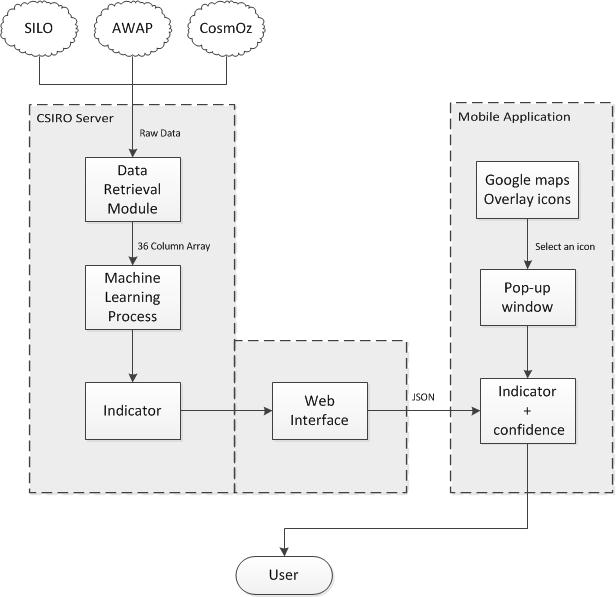
\includegraphics[width=.8\linewidth]{Sch_system.jpg}
  \caption{}
  \label{fig:sub1}
\end{subfigure}%
\begin{subfigure}{.3\textwidth}
  \centering
  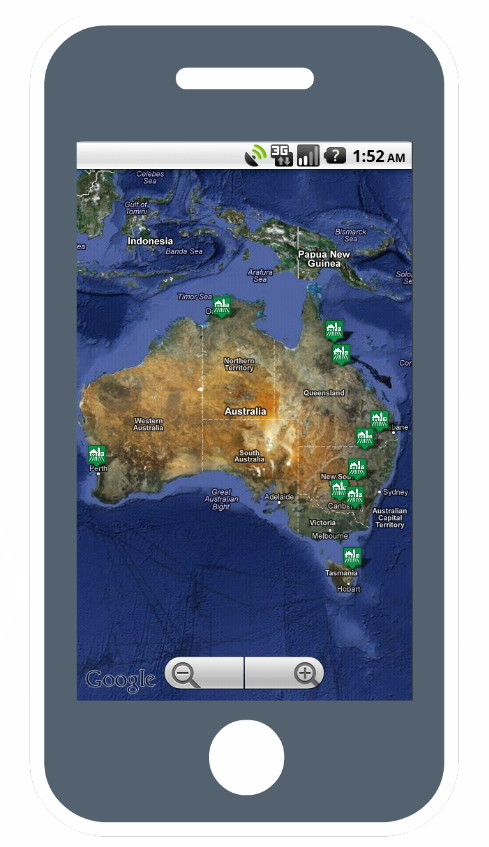
\includegraphics[width=.8\linewidth]{screenshot.jpg}
  \caption{}
  \label{fig:sub2}
\end{subfigure}
\caption{(\ref{fig:sub1}) Schematic diagram of point-based analysis and visualisation system\\ (\ref{fig:sub2}) Screenshot of client-end mobile application}
\label{fig:pointschematic}
\end{figure}
\section{Area-wise Analysis\& Application(Work in Progress)}
As shown in Figure \ref{fig:areaschematic}, an additional data \emph{MODIS VI} provided by NASA, which has no dependency with AWAP data is added to the system. The target in the area-wise analysis is to train a Machine Learning model that can predict the water balance of any given location using historic and spatial data of that region.\\
\newline
This section of the project is still in-progress. The preprocessing and storage facility have been completed, which is essentially the preparation steps. To conduct the analysis, a variety of Machine learning algorithms is going to be implemented and tested, which includes but not limited to \emph{Fuzzy-C-M, K-Means,  self-organizing map(SOM) network, LDA and some ensemble neural network framework etc.}, as well as various water balance models that are in place. The historic data is going to be randomised in order to cross validate the precison of the model's output. The algorithm presents the highest probable results will be used for further development. The Houston salad farm located in Tasmania will be used as a case study for the analysis.
\begin{figure}[H]
\begin{center}
	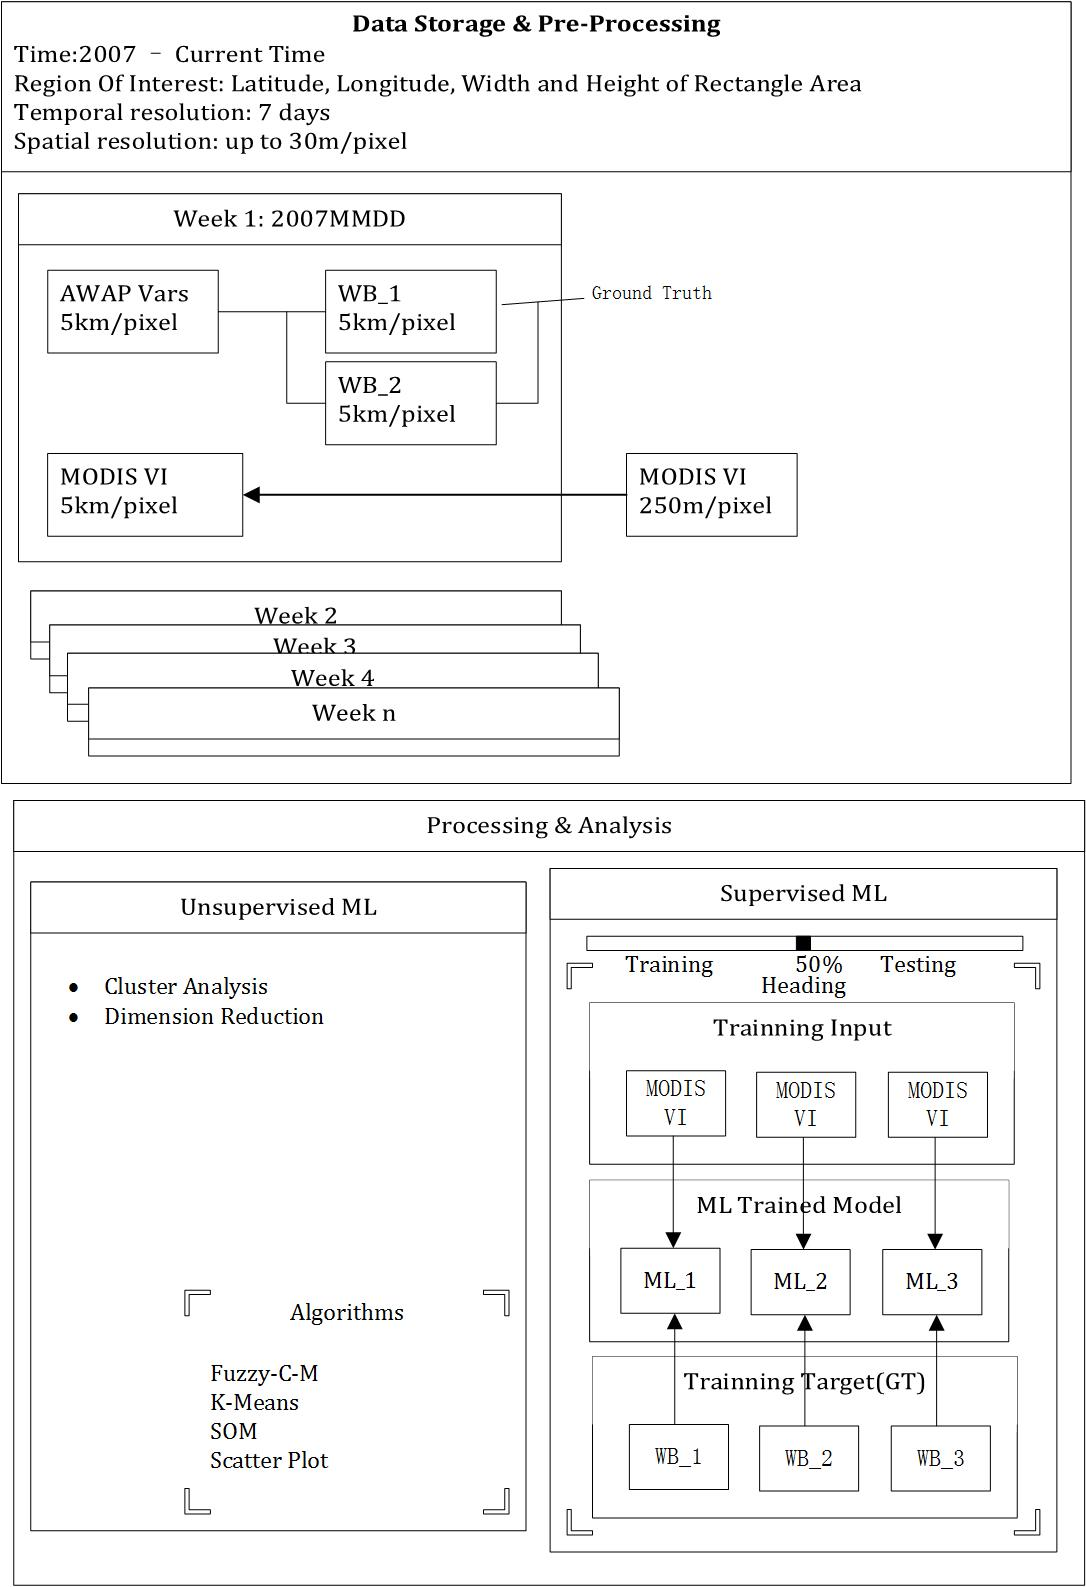
\includegraphics[width = 14cm]{Drawing1.jpg}
	\caption{Schematic diagram of area-wise analysis and visualisation system. Where WB\_n is the various water balance model, ML\_n is the machine learning framework}
	\label{fig:areaschematic}
\end{center}
\end{figure}
\section{Further Development and Conclusion}

At this stage, the single point-based analysis and the mobile application has been finalised and presented in peer reviewed conference. The emphasis of the work is placed on conducting and verify the viability of high resolution spatio-temporal analysis of any arbitrary location using a data driven approach. Most of the fundamental components for the final stage analytics have been completed. The analysis will trial as many potential algorithms and models as the time constrain allows.

\newpage
\appendix

\bibliographystyle{unsrt}
\bibliography{library,manual}	


\end{document}


